% Construction : carré unité de côté 1 en bas à gauche, agrandi de rapport k = 3.
%   Le grand carré, de côté 3, se pave par 3 × 3 = 9 copies du petit.
%   Les longueurs sont multipliées par 3, les aires par 3² = 9.
% SVG : x = 30 + 40x, y = 140 - 40y.
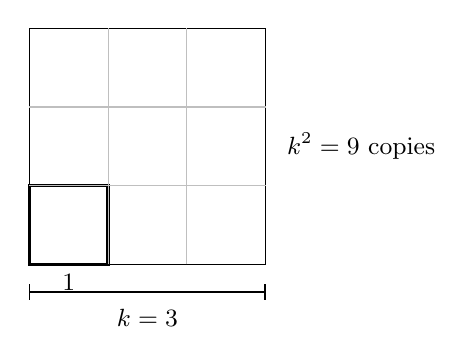
\begin{tikzpicture}[scale=1, every node/.style={font=\small}]
  \draw[very thick] (0,0) rectangle (1,1);
  \draw (0,0) rectangle (3,3);
  \foreach \i in {1,2} { \draw[gray!50] (\i,0) -- (\i,3); \draw[gray!50] (0,\i) -- (3,\i); }
  \node[below] at (0.5,0) {$1$};
  \node[below] at (1.5,-0.45) {$k = 3$};
  \draw[|-|] (0,-0.35) -- (3,-0.35);
  \node[right] at (3.15,1.5) {$k^2 = 9$ copies};
\end{tikzpicture}
